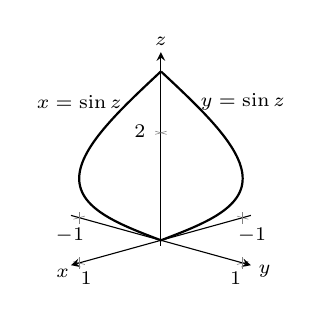
\begin{tikzpicture}[>=stealth]
\begin{axis}%
[width=175pt,tick label style={font=\scriptsize},axis on top,
			axis lines=center,
			view={135}{20},
			name=myplot,
			%xtick=\empty,
			%ytick=\empty,
			%ztick=\empty,
			ymin=-1.1,ymax=1.1,
			xmin=-1.1,xmax=1.1,
			zmin=-.1, zmax=3.5,
			every axis x label/.style={at={(axis cs:\pgfkeysvalueof{/pgfplots/xmax},0,0)},xshift=-3pt,yshift=-3pt},
				xlabel={\scriptsize $x$},
			every axis y label/.style={at={(axis cs:0,\pgfkeysvalueof{/pgfplots/ymax},0)},xshift=5pt,yshift=-2pt},
				ylabel={\scriptsize $y$},
				every axis z label/.style={at={(axis cs:0,0,\pgfkeysvalueof{/pgfplots/zmax})},xshift=0pt,yshift=4pt},
				zlabel={\scriptsize $z$}
			]

%\addplot3[domain=0:180,smooth,y domain=0:360,surf,%fill=white,
%colormap={mp2}{\colormapplaneone},faceted color=black!40,samples=30,samples y=25,very thin,z buffer=sort] ({cos(x)*1.5*cos(y)},{sin(x)*cos(y)},{sin(y)});

\addplot3[domain=0:3.14,,thick,smooth,samples y=0,{\colorone},%surf,%fill=white,
samples=30,] ({0},{sin(deg(x))},{x});

\draw (axis cs: 0,1,3) node {\scriptsize $y=\sin z$};

\addplot3[domain=0:3.14,,thick,smooth,samples y=0,{\colortwo},%surf,%fill=white,
samples=30,] ({sin(deg(x))},{0},{x});

\draw (axis cs: 1,0,3) node {\scriptsize $x=\sin z$};


\end{axis}


\end{tikzpicture}












